\documentclass[12pt]{article}
\usepackage{graphicx}
\usepackage{hyperref}
\usepackage{fancyhdr}
\usepackage{setspace}
\pagestyle{fancy}
\fancyhead{}
\fancyfoot{}
\fancyfoot[C]{-\thepage-}
\fancyfoot[L]{ID:997900158}
\fancyfoot[RO]{MPM406 - Random Clinical Trial}
\renewcommand{\footrulewidth}{0.4 pt}
\renewcommand{\headrulewidth}{0 pt}

\hypersetup{colorlinks = true, linkcolor = blue, citecolor = blue}
\title{Investigation into the effect of growing food onsite on the incidence of cryptosporidiosis in California Ranching households}
\author{Student ID: 997900158}
\date{\today}
\begin{document}
	\maketitle
	\begin{abstract}
		This cohort study's objective was to investigate the relationship between California ranchers growing food onsite and incidence of cryptosporidiosis in their household.
		Ranchers from a CDFA database were sent an initial questionnaire, followed up by a visit from a nurse practitioner to collect information on various household, occupational, and dietary variables.


		Households that grew more than 50\% their food  on site were 3.01 (95\% CI: 2.81 - 3.21)times more likely to experience a cryptosporidiosis event each year than those who did not grow more than 50\% of food onsite.

	\end{abstract}

\onehalfspace
	\section{Introduction} 
		def CVD 
		In 1994, Cardiovascular disease killed a half million women and accounted for over 40\% of all deaths in women, more than all forms of cancer combined\cite{AHA1997}.
		Even though there has been an overall decline in the death rate due to cardiovascular disease in the United States over several decades, the rate of decline is less for women and especially african-american women \cite{Mosca1997}.
		While men are more commonly affected by cardiovascular disease, risk increases rabpidly in women as they age, doubles every decade after age 55\cite{Gordon1978}. 
		It has been shown that reduced circulating ostradiol during menopause increases atherogenic lipids and reduces carotid blood flow, causing increased incidence of athersclerotic cardiovascular disease \cite{Hodis}.
		Menopause is the abcence of a menstural cycle in the previous 12 months, and occurs at an average age of 51 but can range between 45 and 55 years \cite{Gold2012}. 
		Supplamental oestrogen has been used for some time to treat symptoms of menopause and its associated increase in athersclerotic cardiovascular disease risk, however serious side effects ( higher risk of breast cancer, increased blood clots and endometrial cancer) have been documented \cite{Gold2012}.
		Recent research has also questioned the cardiovascular protection associated with menopausal hormonal therapy and concluded no overall benfit to supplamental estrogen overall, and a possible interaction between time of therapy initiation and protection provided \cite{Anderson2004,Prentice2009}.
		Since the initial reasearch questioning the efficacy of menopausal hormonal therapy was completed, there have been numerous innovations in the form and dose of estrogen deliverey have occurred, and it is hypothesised that these new forms/dosing regiemes may provide improved protention.



		This two-by-two factorial radomized clinical trial is designed to assess the effects of intiating estradiol supplementation at diffent doses and different times following the onset of menopause on the risk of athersclerotic cardiovascular disease.
		The study Hypothesis is that initiating estrogen therapy before the onset of menopause is protective of athersclerotic cardiovascular disease, and that a reduced dose of estrogen provides the same protection with reduced side effects.


	\section{Methods} 
		The study population was drawn from women presenting to Kaiser Permanente between 2000-01-01 and 2009-12-31, between the ages of 40 and 50 that were undergoing signs of peri-menopause (last cycle less than 12 months ago, but no regular monthly cycle).
		Kaiser Permanente is a managed care consortium based in northern California. It has almost 15,000 physicians operating in 650 facilities spread over 9 states, and serves nearly 9 million members \cite{Rauber}.
		On identifying a possible study subject, a full physical examination and medical history was taken, and where possible validated with a central database of historical medical records maintained by Kaiser Permanente.
		During this physical examination BP, BMI, and age were measured, and lifdestyle factors such as smoking and phjysical activity levels recorded.
		Blood was also collected during this initial examination and levels of lipoprotiens measured.
		Any woman with a previous hysterectomy, had taken estrogen suppleaments in the past, or had experienced any prolonged angina was disqualified from the study as hysterectomy causes instant menopause at any age, and angina may be a sign of preexisting heart conditions.
		

		Sample size recquirements were calculated using epi-info with a subclinical athersclerotic cardiovascular disease rate of 25\%


		Two factorial design was chosen to allow simountaneus comparison of dose and timing effects, and the use of a very large sample size allowed the assessment of interactions at sufficeint power. 
		The two dose levels chosen were 0.625mg and 0.3mg of conjugated equine estrogens, delivered per os.
		0.625 mg SID PO is the standard therapy currently in use, the lower dose of 0.3mg has been suggested as a way to maximise benefit ( menopause symptoms, CVD,osteoporosis), while minimising harmful side effects (cancer risk, blood clots)  associated with estrogen.
		The two timing levels chosen were initiation of therapy during peri menopause, or initiation 3 years after menopause.
		The use of a two factorial design resulted in 4 study groups, as described in \hyperref[Figure 1]{figure1}.


		The primary study endpoint was progression of subclinical athersclerotic cardiovascular disease defined as an increase in carotid inter-media thickness of more than 0.0035mm per year diagnosed on carotid ultrasound.
		A second study endpoint was clinical athersclerotic cardiovascular disease, which included 


		Patients were randomised using a centralised allocation procedure, with both patient and physician blinded to allocation method. 
		After eligibility was established, an auto generated email containing patient information was sent to a server maintained in the researchers office at Kaiser Permanente's headquarters in Oakland, California. 
		This computer used a schedule of random numners generated from atmoshperic noise \cite{Eddelbuettel2009}  and study participants were allocated to one of the four groups basd on this number.
		The result of this allocation was returned to the physician in an email with a number 1-4 and the appropriate treatment initiated.
		The allocation, general patient details, and source and timsetamp of the allocation request were recorded and compared to doctors own records of assignment to ensure accuracy.

		
		Patients had annual checkups with their Kaiser Permanente physician during the study period.
		During this examination, a standard examination and history was performed, as well specific questions relating to the onset of menopause, symptoms experienced during the year, and any incidence of angina or clinical cardiovascular disease.
		Side effects of estrogen therapy monitored included cancer (breast, colon, endometrial), and clotting events (Deep Vein Thrombosis, Ischaemic stroke)
		All women had their responses checked against actual medical history, improving accuracy of data and minimising recall bias.
		To assess the progression of subclinical athersclerotic cardiovascular disease, women had a carotid ultrasound to measure carotid arterey intima-media thickness.
		The thickness of carotid arterey intima-media was recorded and compared to previous measurements to assess disease progression.
		This intervention was well tolerated as women were presenting to their health professional for an annual checkup anyway, and the Carotid ultrasound is quick and non-invasive
		In addition, the quality of these measurments were maintained by using a trained ultrasonographer at each of the Kaiser Permanente facilities.
		Before the beginnning of enrollment, these ultrasonographers were trained at a central location on a standard protocol for taking measurements, and the inter-observer agreement assessed by completing an examination of 5 test subjects.


	\subsection{Statistical Evaluation}
		Cox proportional hazard models were used with time to event as response and various covariates discussed above as predictors, with a household level random effect included.
		The baseline hazard was modified to follow a weibull distribution to reflect the time dependence of risk for cryptosporidiosis, with an increased risk occurring with the presence of young calves following calving start date. 
		Incidence density rates were calculated for all strata of the covariates with findings indicated in \hyperref[table2]{Table 2}.
		All statistical analysis were completed in R \cite{RCoreTeam2012}.



	\section{Results}

		
		The rates of diagnosis on each ultrasonographer were compared to ensure inter-observer agreement.
		As each ultrasonographer completed many measurements, each individual observer distribution was compared to the average distribution of all observers, to determine if any one observer was over or under measuring carotid inter-media thickness.
		The interobserver correlation was above 90\% and no single observer consistently over or under measured carotid inter-media thickness.
		The measuremnents between ultrasonographers were compared 


	\section{Discussion} 


	\subsection{Strengths and Limitations}
		Data quality was a strenth of this study.
		Cross validating the patients oral medical histories with the actual recorded histories from the Kaiser Permanente central databases ensures accuracy and reduces recall bias.
		Allocation of participants to study groups was entirely random and repeatable, and the comparison of allocation and actual treatment records allowed analysis to be undertaken on an accurate intention to treat basis. 

		Blinding 


		A potential limitation of this study was the selection of study participants from Kaiser Permanente hopitals.
		Rates of insurance are correlated with Socio economic status and Education level, both factors that are also associated with use of menopausal hormonal therapy.
		There may be some relationship between lifestyle factors/SES and progression of athersclerotic cardiovascular disease, and out attemp to control for these factors (correcting for smoking and activity levels) may be insufficient.

		
	\section{Figures}

\begin{figure*}[h!]
	\centering
	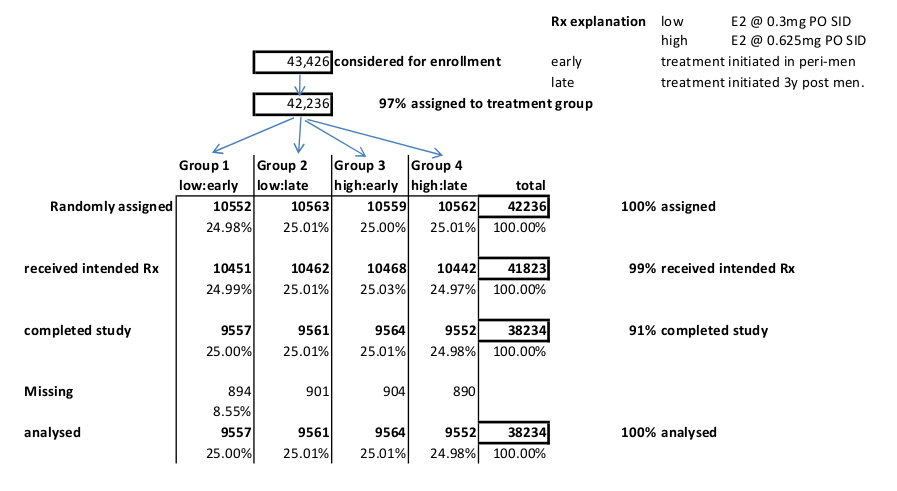
\includegraphics[scale=0.3]{figure1.jpg}
	\caption{Flow Diagram showing proposed Biological Rationale for study, including exposure, outcome and covariates }
	\label{figure1}
\end{figure*}

\begin{figure*}[h!]
	\centering
	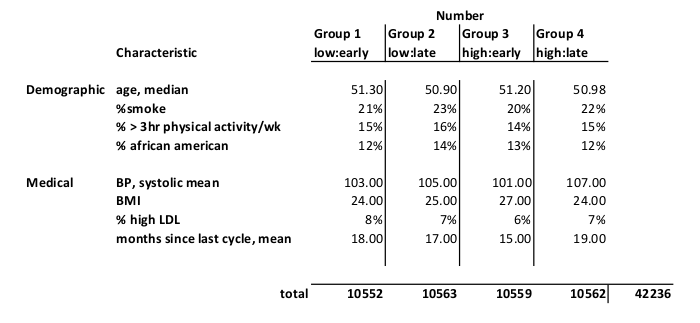
\includegraphics[scale=0.5]{table1.jpg}
	\caption{Characteristics of study participants and sample size calculations.}
	\label{table1}
\end{figure*}
 
\begin{figure*}[h!]
	\centering
	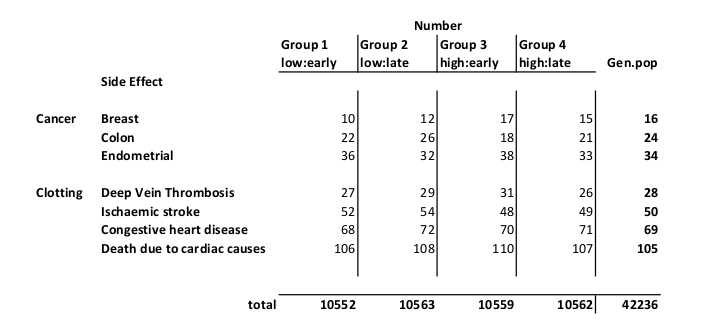
\includegraphics[scale=0.5]{table2.jpg}
	\caption{Risk Ratios (RR) for the association between growing food onsite and cryptosporidiosis.}
	\label{table2}
\end{figure*}

\begin{figure*}[h!]
	\centering
	\includegraphics[scale=0.6]{sample.jpg}
	\caption{Sample size function and calculation output from R. Calculations agrees with Epi Info when continuity correction was applied.}
	\label{sample}
\end{figure*}

\clearpage
\bibliographystyle{unsrt}
\bibliography{wom}



\end{document}

%%%%%

% interactoins - 
%% make streamlined as possible. but need at least one confounder, not necc any interactions, can say did not find any (kim paper for technique - none stat sig so not included). potential effect modify - wualitative. 
% if include need to show OR with and without interactions.
% table 1 - cats in study,. throw in other factors that wont include - make them the same. e.g. age w exposure outcome and not on causal path. - no sig p value. 
% fig 1 - exposure b \emph{Bartonella sp.} , outcome ev.

% diagram bartonella causing uveitis, age associated w bartonella and uveitis (double ended arrow.) then show in table.( anythign in table that same do not need to have in diagram.
